\newpage
\section{Extending our Functionality}
\genHeader

% Remember, this is relevant for BOTH specifications.

% \emph{Introduce the problem: four partitions. Integrator doesn't help, what do? Protocol! Explain what went wrong, new rule! Run again, show protocol round
% two, and look! it runs fine.}

% Introduce problem: we want four partitions. Add one - woah, it doesn't work! Let's try the integrator. Doesn't help. Chat about the protocol. Lets implement a
% new rule!
% protocol Splash

% vis rule

% tex rule

% Run it again! It works! BRILLIANT. Show in protocol.

At this point, we now have a working TGG transformation for Dictionary into box with three partitions, and a box with \emph{precisely} three partitions into a
Dictionary. The only potential problem here is that exactly three partitions in a LearningBox is rather unrealistic as a proper studying tool. After all, the
more you need to practice a subject, the more cards and partitions you should have so you can be quizzed again and again.

Given that we have three partition and a rule to transform these, lets add a fourth partition to our source graph and see if it our TGG will at least complete
a partial transformation. Modify your \texttt{source.xmi} until it resembles Fig.~\ref{fig:fourthPartitionStart}.

\begin{figure}[htbp]
\begin{center}
  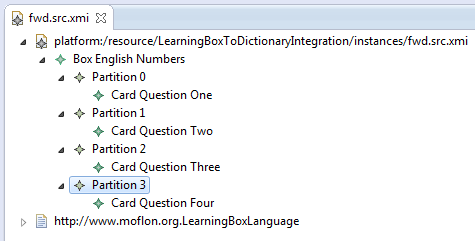
\includegraphics[width=0.7\textwidth]{eclipse_fillFourthPartition}
  \caption{caption}
  \label{fig:fourthPartitionStart}
\end{center}
\end{figure}

Don't forget to set its \texttt{previous} value to \texttt{partition0}, and the \texttt{next} value of \texttt{Partition 2} to \texttt{Partition3}.

Save and run TGGMain.

%FailImage

Doesn't work! Let's check the integrator.

{\bf integrator stuff here; where does it fail}


Doesn't help - let's check the protocol!


{\bf protocol stuff here; precisely where/WHY it fails}

Even though there was a solution to the first threee, there was no way it could have connected number 4 successfully, resulting
in a dangling edge, which fujaba does not allow \ldots why didn't at least the first set of card from partitions 0, 1, 2. Work? Dangling edges - predicts that there
will be no way to repair it, so it ends te whole operation.

While we addressed in index issue in our implemenation code (anzthing above 2 would be assigned as index 2), that only took care of the attribute, not the
actual object. Lets consider just extending our current rule so it could handle a fourth card \ldots It would be as simple as including
another partition in our rule and connecting it proberly. But what if we wanted a fith? a sixth?  This obviously won't work -- there will always be an n+1
partition that needs to be resolved.

Instead, let's create a new rule so that the TGG can check both. After all, the protocol is bound to try EVERY possilbilty before continuing. that means, if
the first rule fails, it will try to apply this one, and it will succeed.

\jumpDual{allCards vis}{allCards tex}

\newpage
\hypertarget{allCards vis}{}
\subsection{AllOtherPartitionsRule}
\genHeader

\begin{itemize}

\item[$\blacktriangleright$] Create a new rule \texttt{AllOtherPartitionsRule}, and complete it according to \Cref{fig:ea_AllOtherPartitionsRuleComplete}.


\begin{figure}[htbp]
\begin{center}
  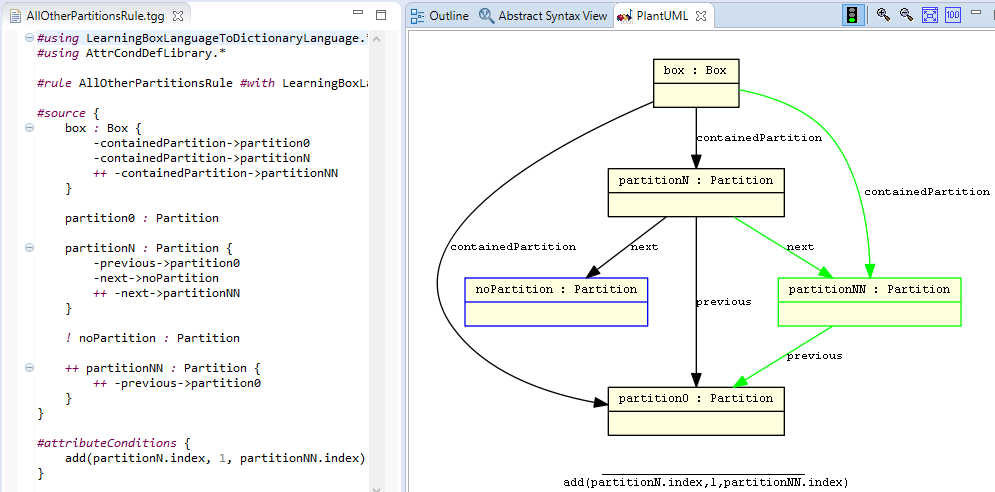
\includegraphics[width=\textwidth]{ea_AllOtherPartitionsRule}
  \caption{The completed \texttt{AllOtherPartitionsRule}}
  \label{fig:ea_AllOtherPartitionsRuleComplete}
\end{center}
\end{figure}

\item[$\blacktriangleright$] As you can see, this rule doesn't assume to know the final \texttt{partition} in the transformation. 
It matches the \texttt{n}th partition as the partition without any next partition, then connects a new \texttt{n+1}th partition to \texttt{n} and \texttt{partition0} (clear as every partitions previous is \texttt{partition0}).
Note that TGG transformations assume that the models are valid, i.e., have the expected structure (in our case meaning that the learning box is correctly ``wired'').\footnote{This should actually be formalised with a set of metamodel constraints that must be checked before a transformation is run, but we've omitted this here to simplify things.}  
Remember that ``blue'' means ``negative''.

\item[$\blacktriangleright$] Generate code for your improved TGG and re-run the transformation. 
It should work now without any error message.
Inspect the protocol to understand what happened.

\item[$\blacktriangleright$] Go ahead and add as many \texttt{partition}s and \texttt{card}s as you like to your model instance.
Your TGG is now also able to handle a \texttt{box} with any number of \texttt{partition}s beautifully.
For five partitions all with cards, the protocol gets quite interesting and is no longer a flat tree.
Try it out! 

\end{itemize}



%%% Local Variables: 
%%% mode: latex
%%% TeX-master: "../src/TGG_mainFile"
%%% End: 


\newpage
\hypertarget{allCards tex}{}
\subsection{AllOtherCardsRule}
\texHeader

\begin{itemize}

\item[$\blacktriangleright$] Right click on the \texttt{rules} folder again and create \texttt{AllOtherCardsRule}. Complete the rule until your file resembles
Fig.~\ref{fig:eclipse_allOtherCardsRule}.

\vspace{0.5cm}

\begin{figure}[htbp]
\begin{center}
  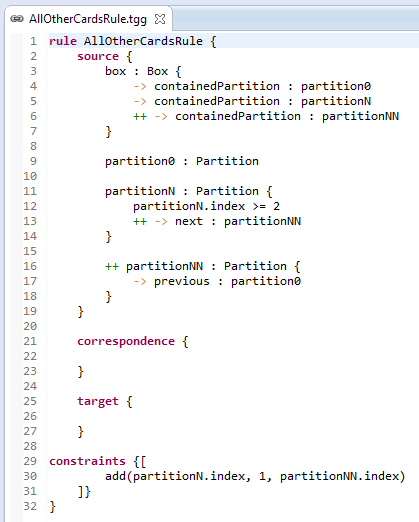
\includegraphics[width=0.7\textwidth]{eclipse_allOtherCardsRule}
  \caption{A complete \texttt{AllOtherCardsRule}}
  \label{fig:eclipse_allOtherCardsRule}
\end{center}
\end{figure}

\item[$\blacktriangleright$] You'll notice that \texttt{box} and \texttt{partition0} have been established as `black' objects -- this rule may only be evaluated
when these objects are already known (and simply need to be adjusted), so we can use their values from the context of the transformation.

\vspace{0.5cm}

\item[$\blacktriangleright$] A second partition, \texttt{partitionN}, has also been established from the context. It represents the \texttt{n}th or last
partition in a \texttt{box} (with an index of 2 or higher), whose \texttt{next} reference will be updated in order to provide an access
link to the newest element, \texttt{partitionNN}.

\newpage

\item[$\blacktriangleright$] Given that the \texttt{add(a,b,c)} syntax is \texttt{a+b=c}, the sole constraint of this rule sets the \texttt{index} of the
\texttt{n+1}th partition so that the \texttt{partition}s are still listed in order.

\vspace{0.5cm}

\item[$\blacktriangleright$] That's it! Save and build your package explorer, then run the TGG again with the `extra' \texttt{partition} to confirm it worked!
You are now free to add as many \texttt{partition}s and \texttt{card}s to \texttt{source.xmi} -- the transformation is now able to elegantly handle them all.

\vspace{0.5cm}

\item[$\blacktriangleright$] Be sure to check out how this rule is implemented in eMoflon's visual specification with Fig.~\ref{fig:ea_allOtherCardsRule} from
the previous section.

\end{itemize}


\newpage
\section{The Protocol Explained}
\genHeader

% files are saved and built/refereshed in the Eclipse workspace.

Now that everything is working correctly, let's return to one of the generated protocol files and quickly review what happens in greater detail. Though it looks
scary, this file can prove to be useful if the integrator was ever to fail again, or if you simply wanted to know more detail about what happened during the
transformation process.

\ldots

